\documentclass[11pt]{scrartcl}
\usepackage{graphicx}
\graphicspath{{./}}
\usepackage[sexy]{evan}
\usepackage[normalem]{ulem}
\usepackage{hyperref}
\usepackage{mathtools}
\hypersetup{
    colorlinks=true,
    linkcolor=blue,
    filecolor=magenta,      
    urlcolor=cyan,
    pdfpagemode=FullScreen,
    }
\usepackage[most]{tcolorbox}
\renewcommand{\dangle}{\measuredangle}

\renewcommand{\baselinestretch}{1.5}

\addtolength{\oddsidemargin}{-0.4in}
\addtolength{\evensidemargin}{-0.4in}
\addtolength{\textwidth}{0.8in}
% \addtolength{\topmargin}{-0.2in}
% \addtolength{\textheight}{1in} 


\setlength{\parindent}{0pt}

\usepackage{pgfplots}
\pgfplotsset{compat=1.15}
\usepackage{mathrsfs}
\usetikzlibrary{arrows}

\title{Miscellaneous Geometry - OSN SD}
\author{Azzam Labib (IG: haxuv.world)}
\date{7 May 2024}
\begin{document}
\maketitle

\begin{enumerate}
\item In the diagram below, points $A, B, C$ and $D$ are the midpoints of the sides of a square. If the area of the largest square below is $390\ cm^2$, find the area of the shaded region.
\begin{figure}[h]
\centering
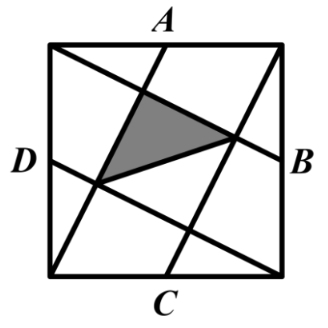
\includegraphics[width=0.2\textwidth]{StarGen/0Figure/shaded-chopped-rectangle.png}
\end{figure}

\vspace{4cm}\item In the rectangle $ABCD$, point $E$ is on the side $AB$ and point $F$ is on the side $AD$ such that $BE = \frac{1}{3} AE$ and $DF = \frac{2}{5} AD$. What is the ratio of areas of $ABCD$ and $FEBCD$?
\begin{figure}[h]
\centering
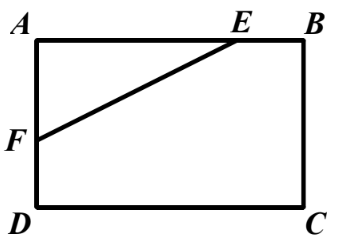
\includegraphics[width=0.2\textwidth]{StarGen/0Figure/chopped-rectangle.png}
\end{figure}

\vspace{6cm}\item Sembilan lingkaran kongruen terletak di dalam persegi seperti terlihat pada gambar. Jika keliling sebuah lingkaran $ 62,8\ cm $ dengan $ \pi = 3,14 $, maka luas daerah yang diarsir adalah ...$ cm^2 $
\begin{figure}[h]
\centering
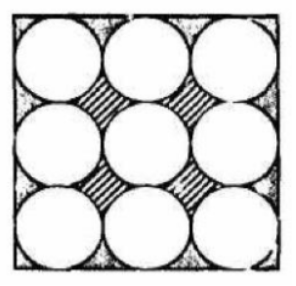
\includegraphics[width=0.2\textwidth]{StarGen/0Figure/9-lingkaran.png}
\end{figure}

\vspace{6cm}\item Perhatikan gambar berikut Jika setiap persegi kecil memiliki luas $ 1\ satuan $, luas daerah tertutup yang dibatasi oleh busur-busur lingkaran di bawah adalah
\begin{figure}[h]
\centering
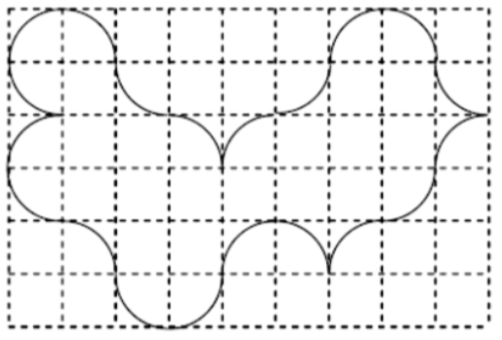
\includegraphics[width=0.4\textwidth]{StarGen/0Figure/curly-path.png}
\end{figure}

\vspace{6cm}\item Pada gambar yang ditunjukkan di bawah, ABC dan AEB merupakan setengah lingkaran. F merupakan titik tengah dari AC dan $ AF = 4 $. Berapakah luas daerah yang diarsir...?
\begin{figure}[h]
\centering
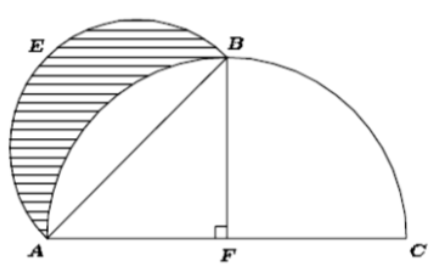
\includegraphics[width=0.4\textwidth]{StarGen/0Figure/2-setengah-lingkaran-sabit.png}
\end{figure}

\vspace{6cm}\item Jika gambar di bawah adalah segi delapan beraturan, maka perbandingan luas antara daerah yang diarsir dan luas segi delapan beraturan adalah ...
\begin{figure}[h]
\centering
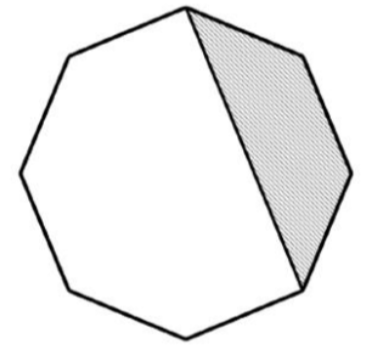
\includegraphics[width=0.2\textwidth]{StarGen/0Figure/luas-diarsir-segidelapan.png}
\end{figure}

\vspace{6cm}\item Perhatikan gambar. Diketahui panjang jari-jari lingkaran $ A = 8\ cm $ dan jari-jari lingkaran $ B = 2\ cm $. Tentukan panjang jari-jari lingkaran $ C $.
\begin{figure}[h]
\centering
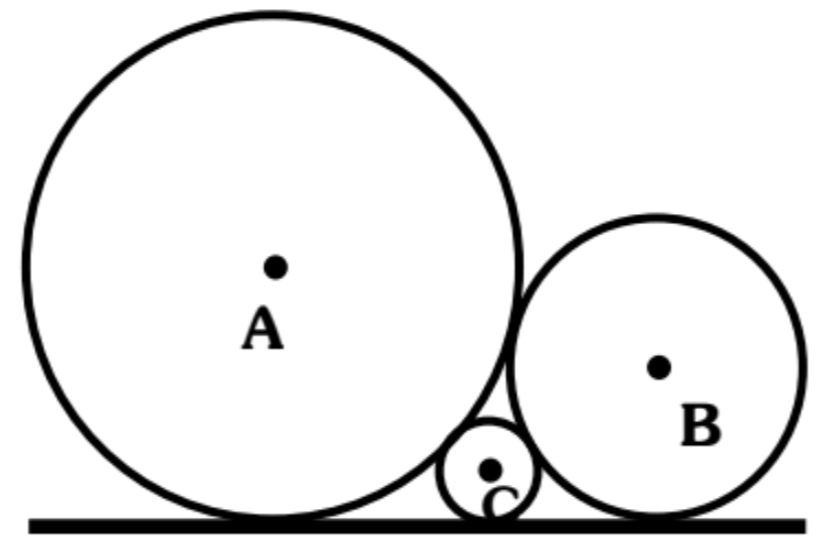
\includegraphics[width=0.4\textwidth]{StarGen/0Figure/3-tangent-circles.png}
\end{figure}


\vspace{6cm}\item Pada gambar di samping $ a, b, c, d $ dan $ e $ berturut-turut menyatakan besar sudut pada titik-titik ujung bintang lima yang terletak pada suatu lingkaran. Jumlah $ a + b + c + d + e = \ldots $
\begin{figure}[h]
\centering
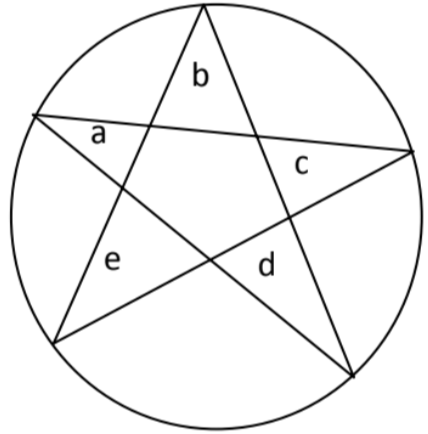
\includegraphics[width=0.3\textwidth]{StarGen/0Figure/star-angle.png}
\end{figure}

\vspace{6cm}\item If a triangle is divided into four pieces with areas as shown, then the area $ x $ equals:
\begin{figure}[h]
\centering
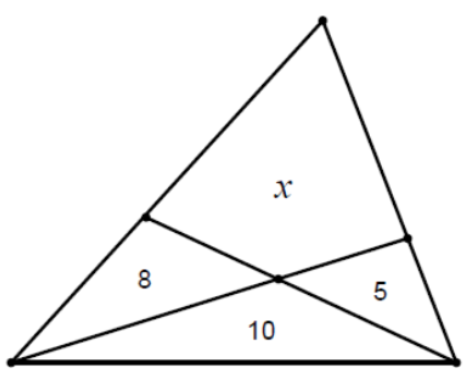
\includegraphics[width=0.35\textwidth]{StarGen/0Figure/area-ratio-classic.png}
\end{figure}

\vspace{6cm}\item Pada $ \triangle ABC $ terdapat titik $ D $ pada $ BC $ sehingga $ BD : DC = 1 : 3 $. Titik $ L $ pada $ AD $ sehingga $ AL : LD = 1 : 4 $. Perbandingan luas $ \triangle ACL $ dan $ \triangle BDL $ adalah ...
\begin{figure}[h]
\centering
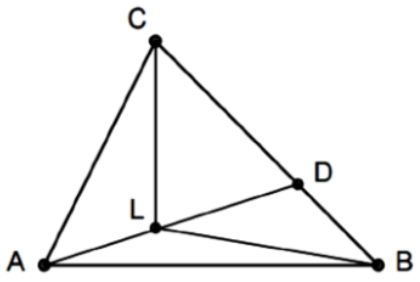
\includegraphics[width=0.4\textwidth]{StarGen/0Figure/area-ratio-triangle-ald.png}
\end{figure}

\end{enumerate}

\end{document}